\begin{answer}

    \begin{figure*}[h]
        \centering
        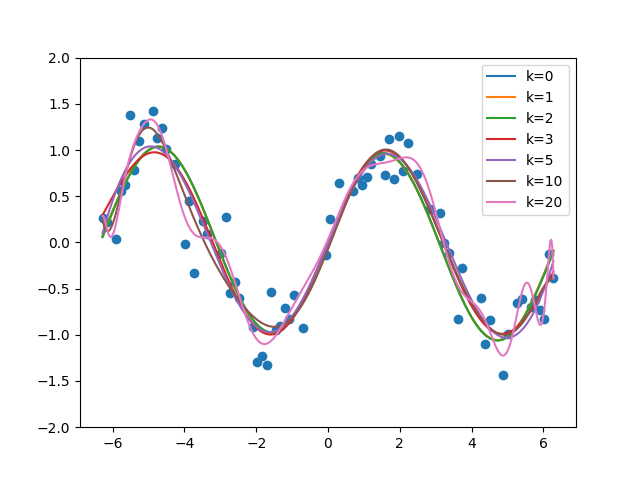
\includegraphics[width=0.8\linewidth]{tex/featuremaps/plot_d.png}
        \caption{plot of degree-k polynomial with sine feature map}
        \label{fig:my_label}
    \end{figure*}
    
    Compare to the previous sub-problem, when we add $sin(x)$ in the feature map, the learnt hypothesis fits more smoothly to the trained data. 

\end{answer}
